% fig_arch.tex: architecture figure (compile with pdflatex; output fig_arch.pdf).
% STIX fonts match the manuscript (cas-dc).
\documentclass[border=2pt]{standalone}
\usepackage{stix}
\usepackage{tikz}
\usetikzlibrary{positioning,fit,calc,arrows.meta}

\definecolor{aam}{HTML}{CDE2FB}
\definecolor{aamedge}{HTML}{2A78D6}
\definecolor{shared}{HTML}{F0EFEC}
\definecolor{sharededge}{HTML}{8A8985}
\definecolor{ink}{HTML}{52514E}

\begin{document}
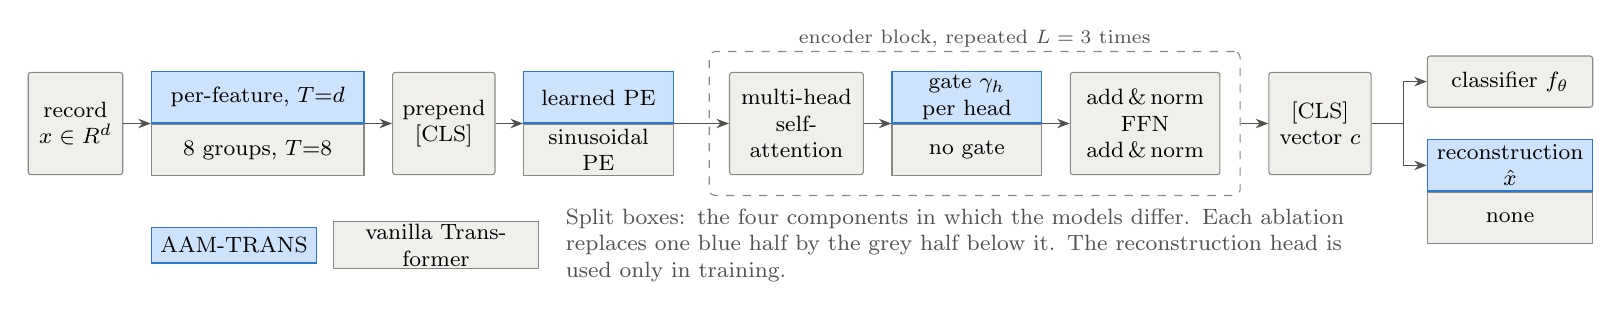
\begin{tikzpicture}[
  >={Stealth[length=1.6mm,width=1.2mm]},
  every node/.style={font=\footnotesize, align=center, inner sep=1pt},
  box/.style={draw=sharededge, fill=shared, rounded corners=1pt,
              minimum height=13mm, minimum width=#1, text width=#1-2mm},
  box/.default=16mm,
  hi/.style={draw=aamedge, fill=aam, minimum height=6.5mm,
             minimum width=#1, text width=#1-2mm},
  lo/.style={draw=sharededge, fill=shared, minimum height=6.5mm,
             minimum width=#1, text width=#1-2mm},
  arr/.style={->, draw=ink, line width=0.5pt},
]
% All boxes are centred on the line y = 0; split boxes have their seam on it.
\def\gap{3.5mm}
\node[box=12mm] (x) at (0,0) {record\\$x\in\mathbb{R}^d$};

\node[hi=27mm, anchor=south west] (tokA) at ($(x.east)+(\gap,0)$) {per-feature, $T{=}d$};
\node[lo=27mm, anchor=north west] (tokV) at ($(x.east)+(\gap,0)$) {8 groups, $T{=}8$};

\node[box=13mm, anchor=west] (cls) at ($(tokA.south east)+(\gap,0)$) {prepend\\{[}CLS{]}};

\node[hi=19mm, anchor=south west] (peA) at ($(cls.east)+(\gap,0)$) {learned PE};
\node[lo=19mm, anchor=north west] (peV) at ($(cls.east)+(\gap,0)$) {sinusoidal PE};

\node[box=17mm, anchor=west] (mhsa) at ($(peA.south east)+(7mm,0)$) {multi-head\\self-attention};

\node[hi=19mm, anchor=south west] (gA) at ($(mhsa.east)+(\gap,0)$) {gate $\gamma_h$ per head};
\node[lo=19mm, anchor=north west] (gV) at ($(mhsa.east)+(\gap,0)$) {no gate};

\node[box=19mm, anchor=west] (ffn) at ($(gA.south east)+(\gap,0)$) {add\,\&\,norm\\FFN\\add\,\&\,norm};

\node[draw=sharededge, dashed, rounded corners=2pt, inner sep=2.5mm,
      fit=(mhsa)(gA)(gV)(ffn)] (enc) {};
\node[anchor=south, font=\scriptsize, text=ink] at (enc.north) {encoder block, repeated $L=3$ times};

\node[box=13mm, anchor=west] (c) at ($(enc.east)+(\gap,0)$) {{[}CLS{]}\\vector $c$};

\node[box=21mm, minimum height=6.5mm, anchor=south west] (clf) at ($(c.east)+(7mm,2mm)$) {classifier $f_\theta$};
\node[hi=21mm, anchor=north west] (rA) at ($(c.east)+(7mm,-2mm)$) {reconstruction $\hat x$};
\node[lo=21mm, anchor=north west] (rV) at (rA.south west) {none};

% Arrows
\draw[arr] (x.east) -- (tokA.south west);
\draw[arr] (tokA.south east) -- (cls.west);
\draw[arr] (cls.east) -- (peA.south west);
\draw[arr] (peA.south east) -- (mhsa.west);
\draw[arr] (mhsa.east) -- (gA.south west);
\draw[arr] (gA.south east) -- (ffn.west);
\draw[arr] (enc.east |- c.west) -- (c.west);
\draw[arr] (c.east) -- ++(4mm,0) coordinate (fork) |- (clf.west);
\draw[arr] (fork) |- (rA.west);

% Legend
\node[hi=21mm, minimum height=4.5mm, anchor=north west] (lA) at ($(tokV.south west)+(0,-6.5mm)$) {AAM-TRANS};
\node[lo=26mm, minimum height=4.5mm, anchor=west] (lV) at ($(lA.east)+(2mm,0)$) {vanilla Transformer};
\node[anchor=west, text=ink, text width=104mm, align=left] at ($(lV.east)+(3mm,0)$)
  {Split boxes: the four components in which the models differ. Each ablation replaces one blue half by the grey half below it. The reconstruction head is used only in training.};
\end{tikzpicture}
\end{document}
